% Appendix Template

\chapter{Lighthouse result table} % Main appendix title

\label{appendix2} % Change X to a consecutive letter; for referencing this appendix elsewhere, use \ref{AppendixX}

\lhead{Lighthouse result tables} % Change X to a consecutive letter; this is for the header on each page - perhaps a shortened title

%\begin{figure}[!h]
%	\centering
%	\begin{adjustbox}{width=\textwidth,totalheight=0.7\textheight}
%		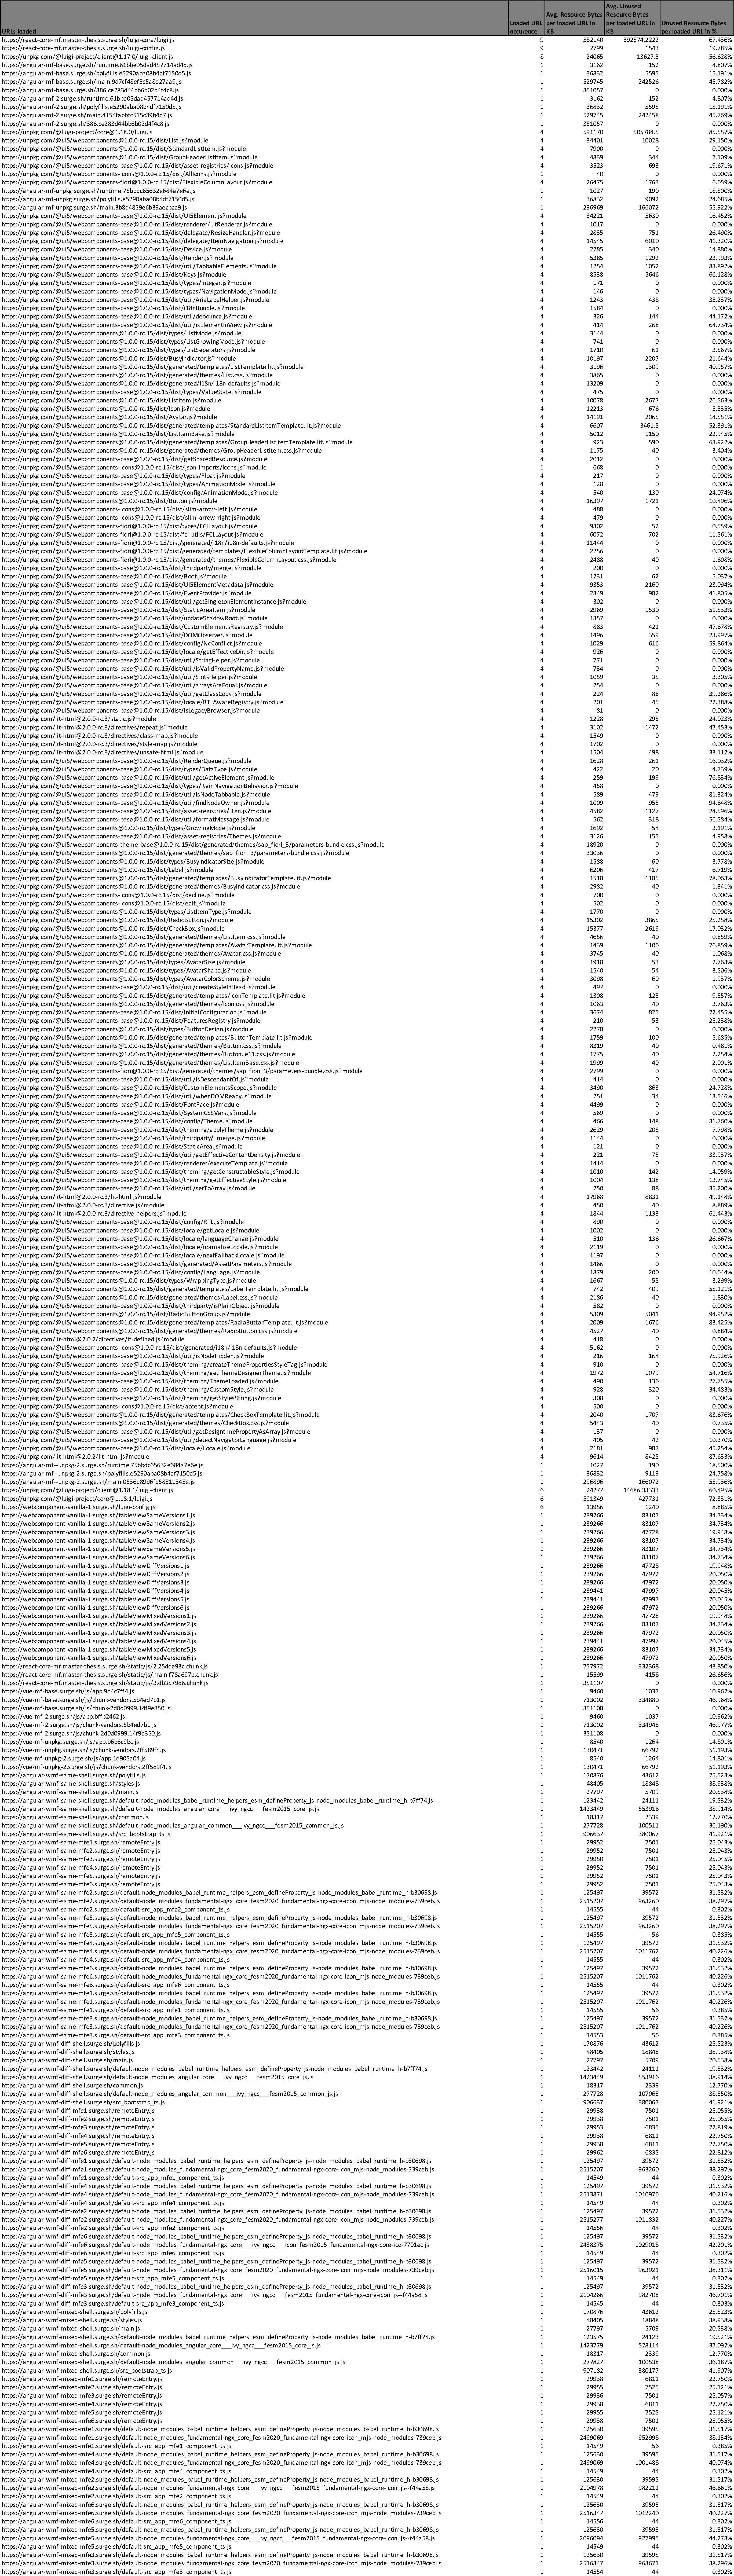
\includegraphics[angle=90]{Figures/lighthouse_json_1.pdf}
%	\end{adjustbox}
%	\caption{Table of numerical results taken from the Lighthouse reports, containing the imported and unused bytes per URL}
%	\label{fig:appendix_2_1}
%\end{figure}
%\newpage
%\begin{figure}[!h]
%	\centering
%	\begin{adjustbox}{width=\textwidth}
%		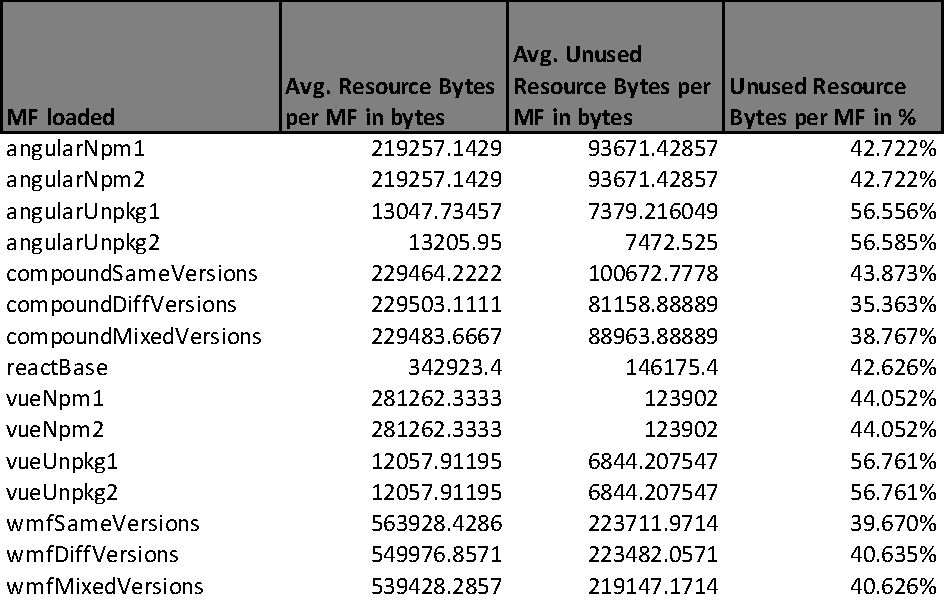
\includegraphics[]{Figures/lighthouse_json_2.pdf}
%	\end{adjustbox}
%	\caption{Table of numerical results taken from the Lighthouse reports, containing the imported and unused bytes per single MF}
%	\label{fig:appendix_2_2}
%\end{figure}
%
%
%
%\begin{figure}[!h]
%	\centering
%	\begin{adjustbox}{width=\textwidth}
%		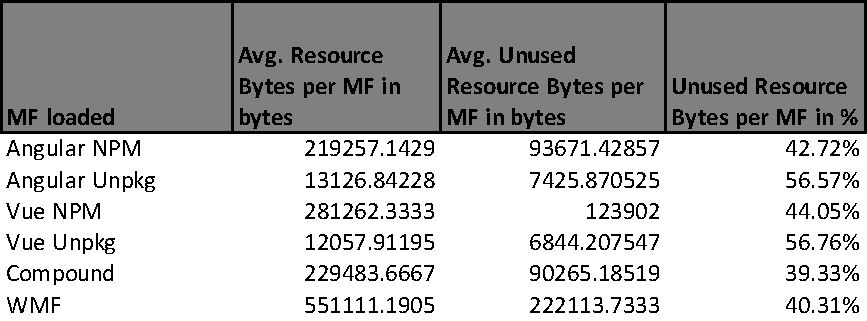
\includegraphics[]{Figures/lighthouse_json_3.pdf}
%	\end{adjustbox}
%	\caption{Table of numerical results taken from the Lighthouse reports, containing the imported and unused bytes per landscape}
%	\label{fig:appendix_2_3}
%\end{figure}